\section{Preventivo}
In questa sezione del documento si può trovare come sono state distribuite le risorse del gruppo nelle varie fasi di lavoro.\\
Inoltre sono illustrate la pianificazione e distribuzione oraria dei ruoli per ogni membro del gruppo, i quali devono:
\begin{itemize}
	\item ricoprire tutti i ruoli durante tutta la durata del progetto;
	\item avere circa le stesse ore produttive alla fine di ogni fase del progetto;
\end{itemize}
Inoltre il verificatore di un determinato task non potrà essere colui che lo ha svolto.\\
Il riferimento alle sigle identificative dei ruoli si può trovare al paragrafo 3.1.3.5 del documento Norme di Progetto.

\subsection{Analisi dei requisiti}
\subsubsection{Preventivo ore}
\begin{table}[h]
	\setlength\extrarowheight{5pt}
	\centering
	\begin{tabularx}{\textwidth}{|c|c|c|c|c|c|c|c|}
		\hline
		\textbf{Nome} & \textbf{Re} & \textbf{Am} & \textbf{An} & \textbf{Pt} & \textbf{Pr}& \textbf{Ve} & \textbf{Ore totali} \\
		\hline
		Ana Lazic &1&4&8&0&0&5&18 \\
		\hline
		Gabriele Da Re &1&8&7&0&0&2&18 \\
		\hline
		Luca Brugnera &1&8&7&0&0&2&18 \\
		\hline
		Matteo Stocco &1&3&7&0&0&7&18 \\
		\hline
		Nicola Sinicato &3&2&8&0&0&5&18 \\
		\hline
		Zhen Wei Zheng &1&3&8&0&0&6&18 \\
		\hline
	\end{tabularx}
	\vspace{10pt}
	\caption{Tabella 10: Distribuzione delle ore durante la fase di Analisi dei requisiti.}
\end{table}
Da inserire figure illustrative.

\vspace{100pt}
\subsubsection{Preventivo costi}
\begin{table}[h]
	\setlength\extrarowheight{5pt}
	\centering
	\begin{tabularx}{\textwidth}{|c|c|c|c|}
		\hline
		\textbf{Ruolo} & \textbf{Costo orario (€)} & \textbf{Costo totale (€)} &\textbf{Ore totali}\\
		\hline
		Responsabile &30&-&- \\
		\hline
		Amministratore &20&-&- \\
		\hline
		Analista &25&-&- \\
		\hline
		Progettista &25&-&- \\
		\hline
		Programmatore &15&-&- \\
		\hline
		Verificatore &15&-&- \\
		\hline
		Totale &-&-&-\\
		\hline
	\end{tabularx}
    \vspace{10pt}
	\caption{Tabella 11: Distribuzione delle ore durante la fase di Analisi dei requisiti.}
\end{table}

\begin{figure}[H]
    \centering
    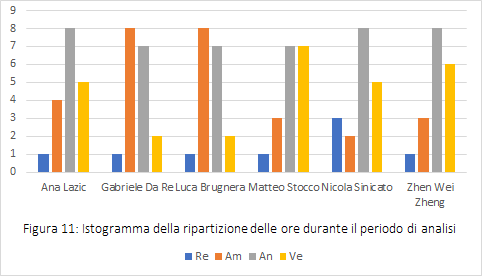
\includegraphics[scale=0.6]{img/grafi preventivo/torta/analisi.PNG}
    \caption{Font Utilizzato}
\end{figure}


